\documentclass{beamer}
\usepackage[T1]{fontenc}
\usepackage[utf8]{inputenc}
\usepackage[french]{babel}
\usetheme{Berlin}

\title{Conception et développement multi-lots / multi-équipes\\ \emph{Application à la supervision à distance d'une ligne de conditionnement temps réel}}
\author{Hexanôme 4203\\ Etienne \textsc{Brodu} \and Martin \textsc{Richard} \and Maxime \textsc{Gaudin} \\ \and Monica \textsc{Golumbeanu} \and Paul \textsc{Adenot} \and Yoann \textsc{Rodière}}

\begin{document}

	\begin{frame}
		\titlepage
	\end{frame}

\section{Introduction}
	\begin{frame}
		Complément de spécifications

		\begin{itemize}	
			\item Les voyants sont reliés à un contrôleur tricolore, une seule
couleur peut être visible à la fois
			\item Le serveur de l'application est hébergé sur le poste
\textit{VxWorks}
			\item Les imprimantes sont sollicitées à tour de rôle afin
d'équilibrer la charge
			\item La date d'un événement est supposée équivalente à la date de
l'enregistrement de l'événement dans les journaux
		\end{itemize}
	\end{frame}

	\begin{frame}
		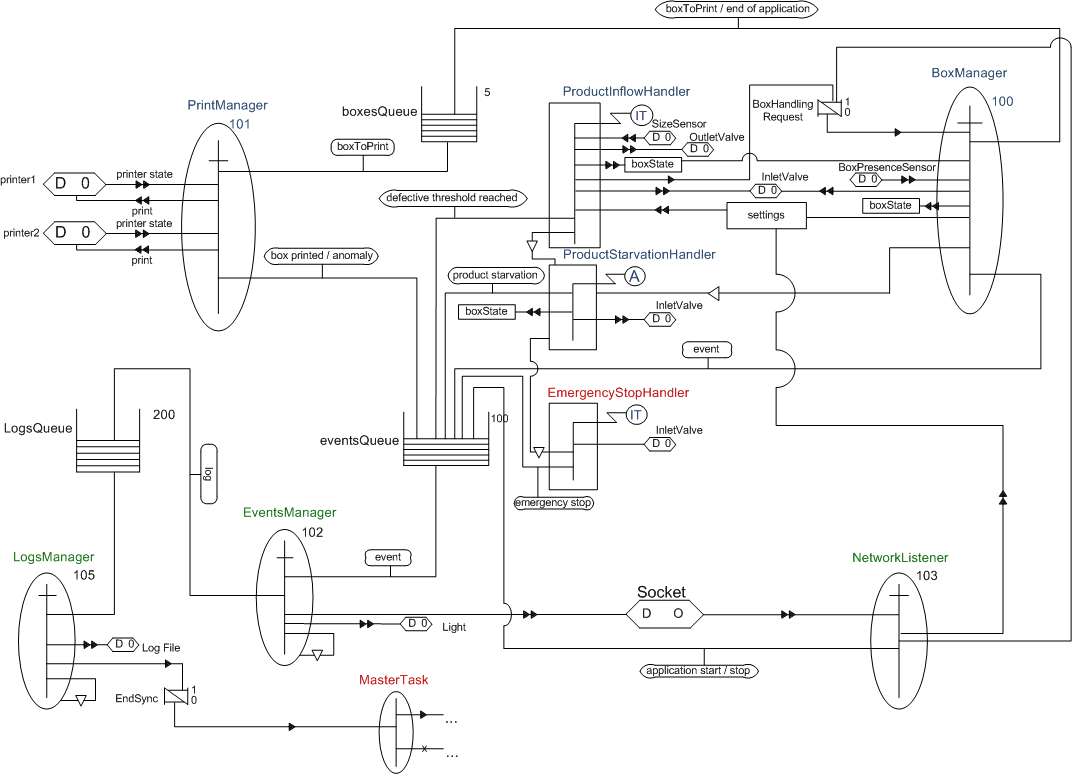
\includegraphics[width=\textwidth]{../../SchemasLCG/schemaGlobal.png}
	\end{frame}

	\begin{frame}
		IHM du poste distant
		connection
	\end{frame}

	\begin{frame}
		IHM du poste distant
		configuration
	\end{frame}

	\begin{frame}
		IHM du poste distant
		log
	\end{frame}

	\begin{frame}
		IHM du poste distant
		erreur \/ warning
	\end{frame}

\section{Binôme 1 (Monica, Yoann)}
	\begin{frame}
\frametitle{Lot 1 : partie métier}
	\begin{figure}
		\centering
		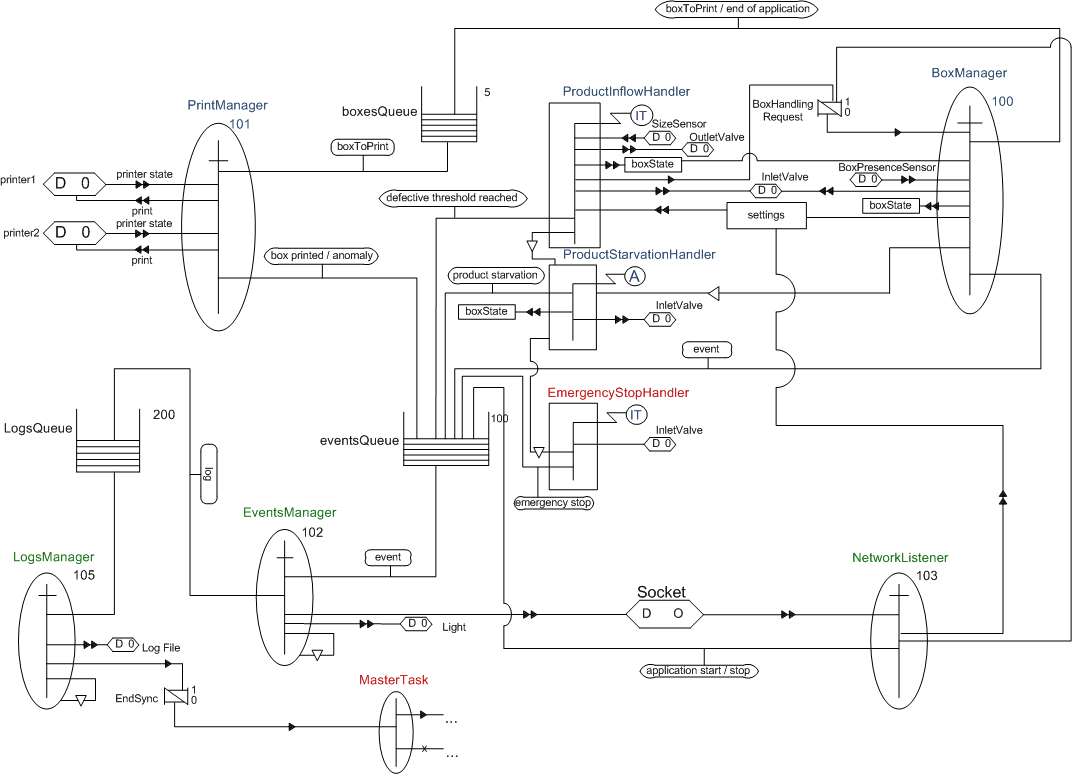
\includegraphics[height=0.8\textheight]{../../SchemasLCG/schemaGlobal.png}
	\end{figure}
	\end{frame}

\subsection{Gestion du remplissage}
	\begin{frame}
	\begin{figure}
		\centering
		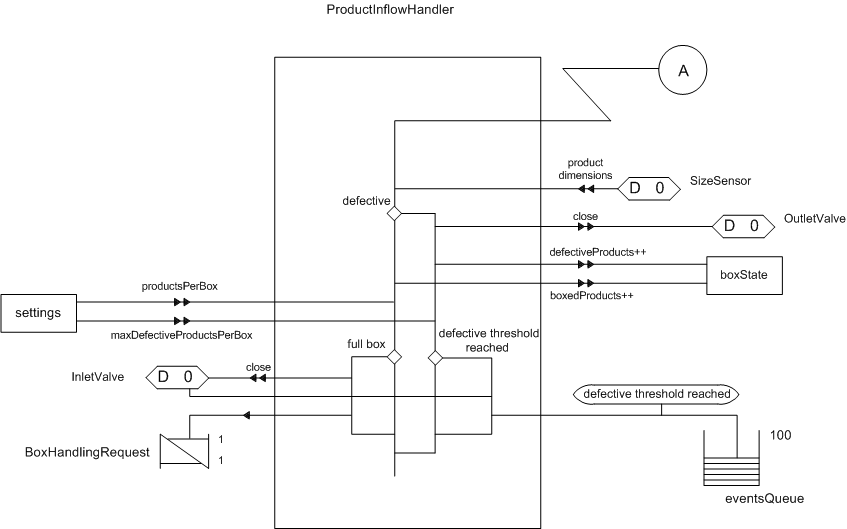
\includegraphics[width=0.9\textwidth]{../../SchemasLCG/ProductInflowHandler.png}
	\end{figure}
	\end{frame}

	\begin{frame}
	\begin{figure}
		\centering
		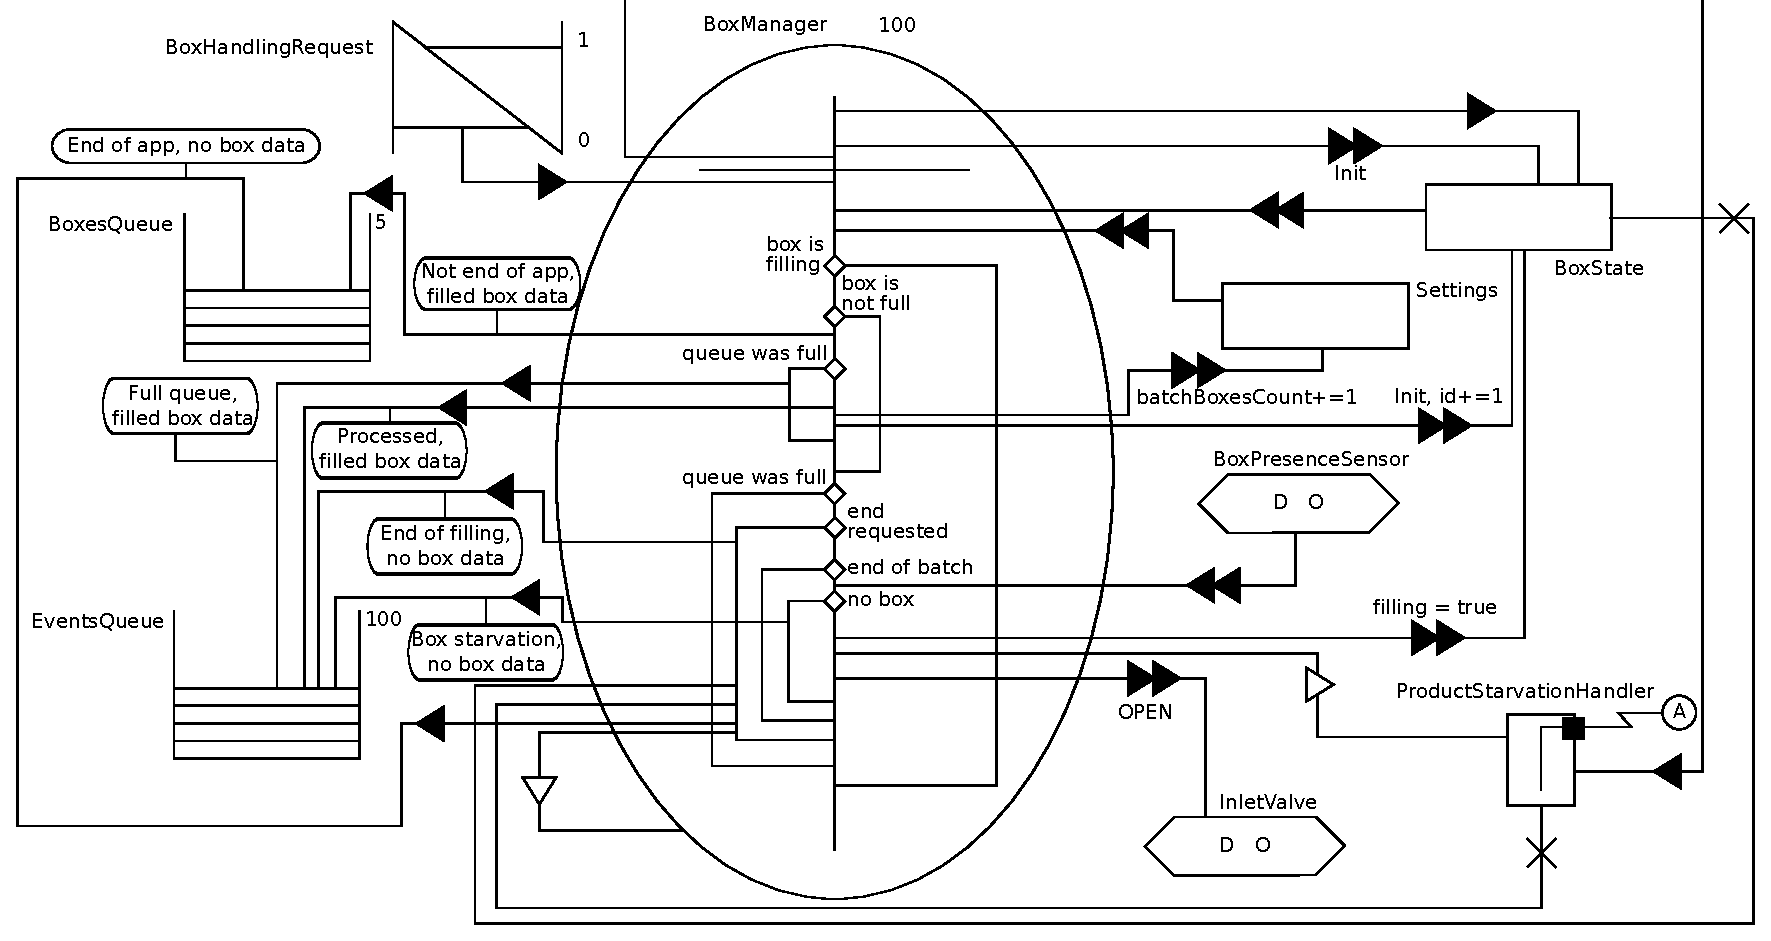
\includegraphics[width=\textwidth]{../../SchemasLCG/BoxManager.pdf}
	\end{figure}
	\end{frame}

	\begin{frame}
	\begin{figure}
		\centering
		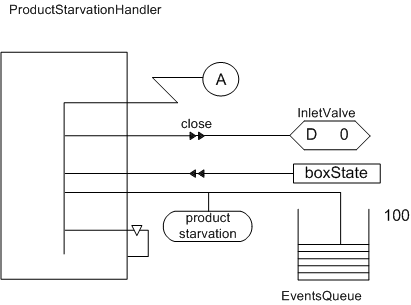
\includegraphics[width=0.7\textwidth]{../../SchemasLCG/ProductStarvationHandler.png}
	\end{figure}
	\end{frame}

\subsection{Gestion de l'impression}
	\begin{frame}
	\begin{figure}
		\centering
		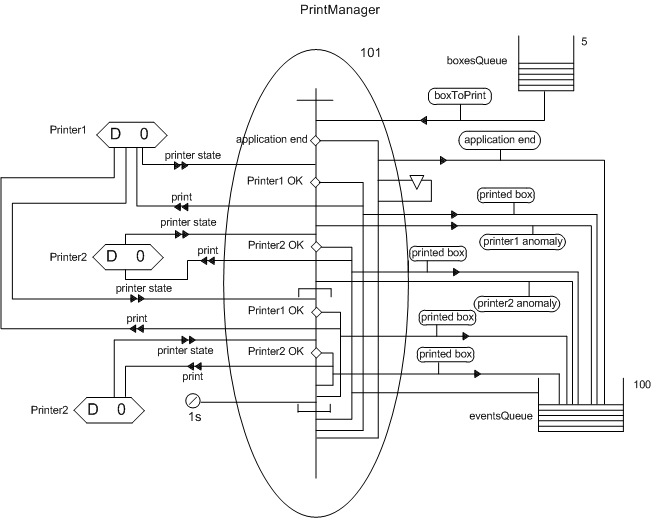
\includegraphics[width=0.85\textwidth]{../../SchemasLCG/PrintManager.png}
	\end{figure}
	\end{frame}

\section{Binôme 2 (Paul, Maxime)}
	\begin{frame}
		\begin{center}
			\frametitle{Lot 2 : réseau, journalisation, gestion des évènements.}
			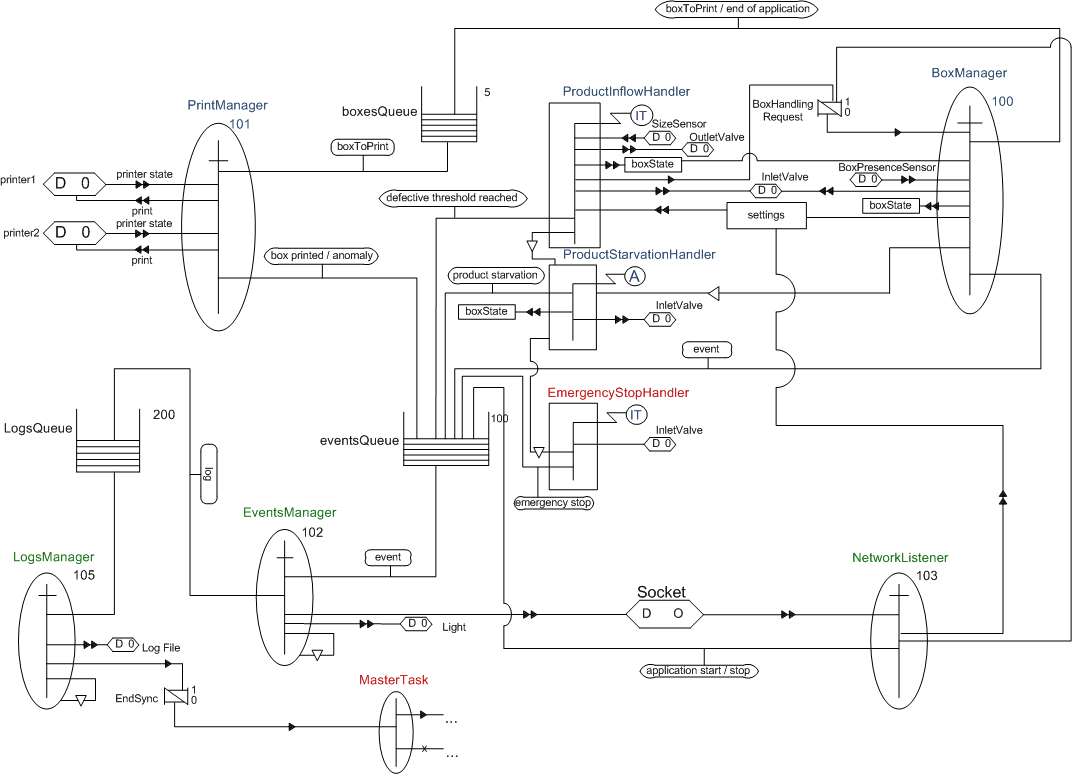
\includegraphics[height=0.8\textheight]{../../SchemasLCG/schemaGlobal.png}
		\end{center}
	\end{frame}

	\begin{frame}
	    \begin{block}{Choix}
		  \begin{itemize}
		      \item Protocole \texttt{plain text}.
		      \item Séparateur : retour chariot.
		      \item 9 commandes différentes dans les deux sens.
		  \end{itemize}
	    \end{block}
	\end{frame}

	\subsection{Protocole en entrée}
	\begin{frame}
		\begin{enumerate}
		    \item \texttt{RESUME} : reprise sur erreur.
		    \item \texttt{STOP} : arrêt du système après les cartons courants.
		    \item \texttt{CONFIG} : 5 valeurs chiffrées pour configurer le système.
		    \item \texttt{LAUNCH} : lancer le système.
		\end{enumerate}
	\end{frame}

	\begin{frame}
	    \frametitle{LCG : Réseau, en entrée}
	    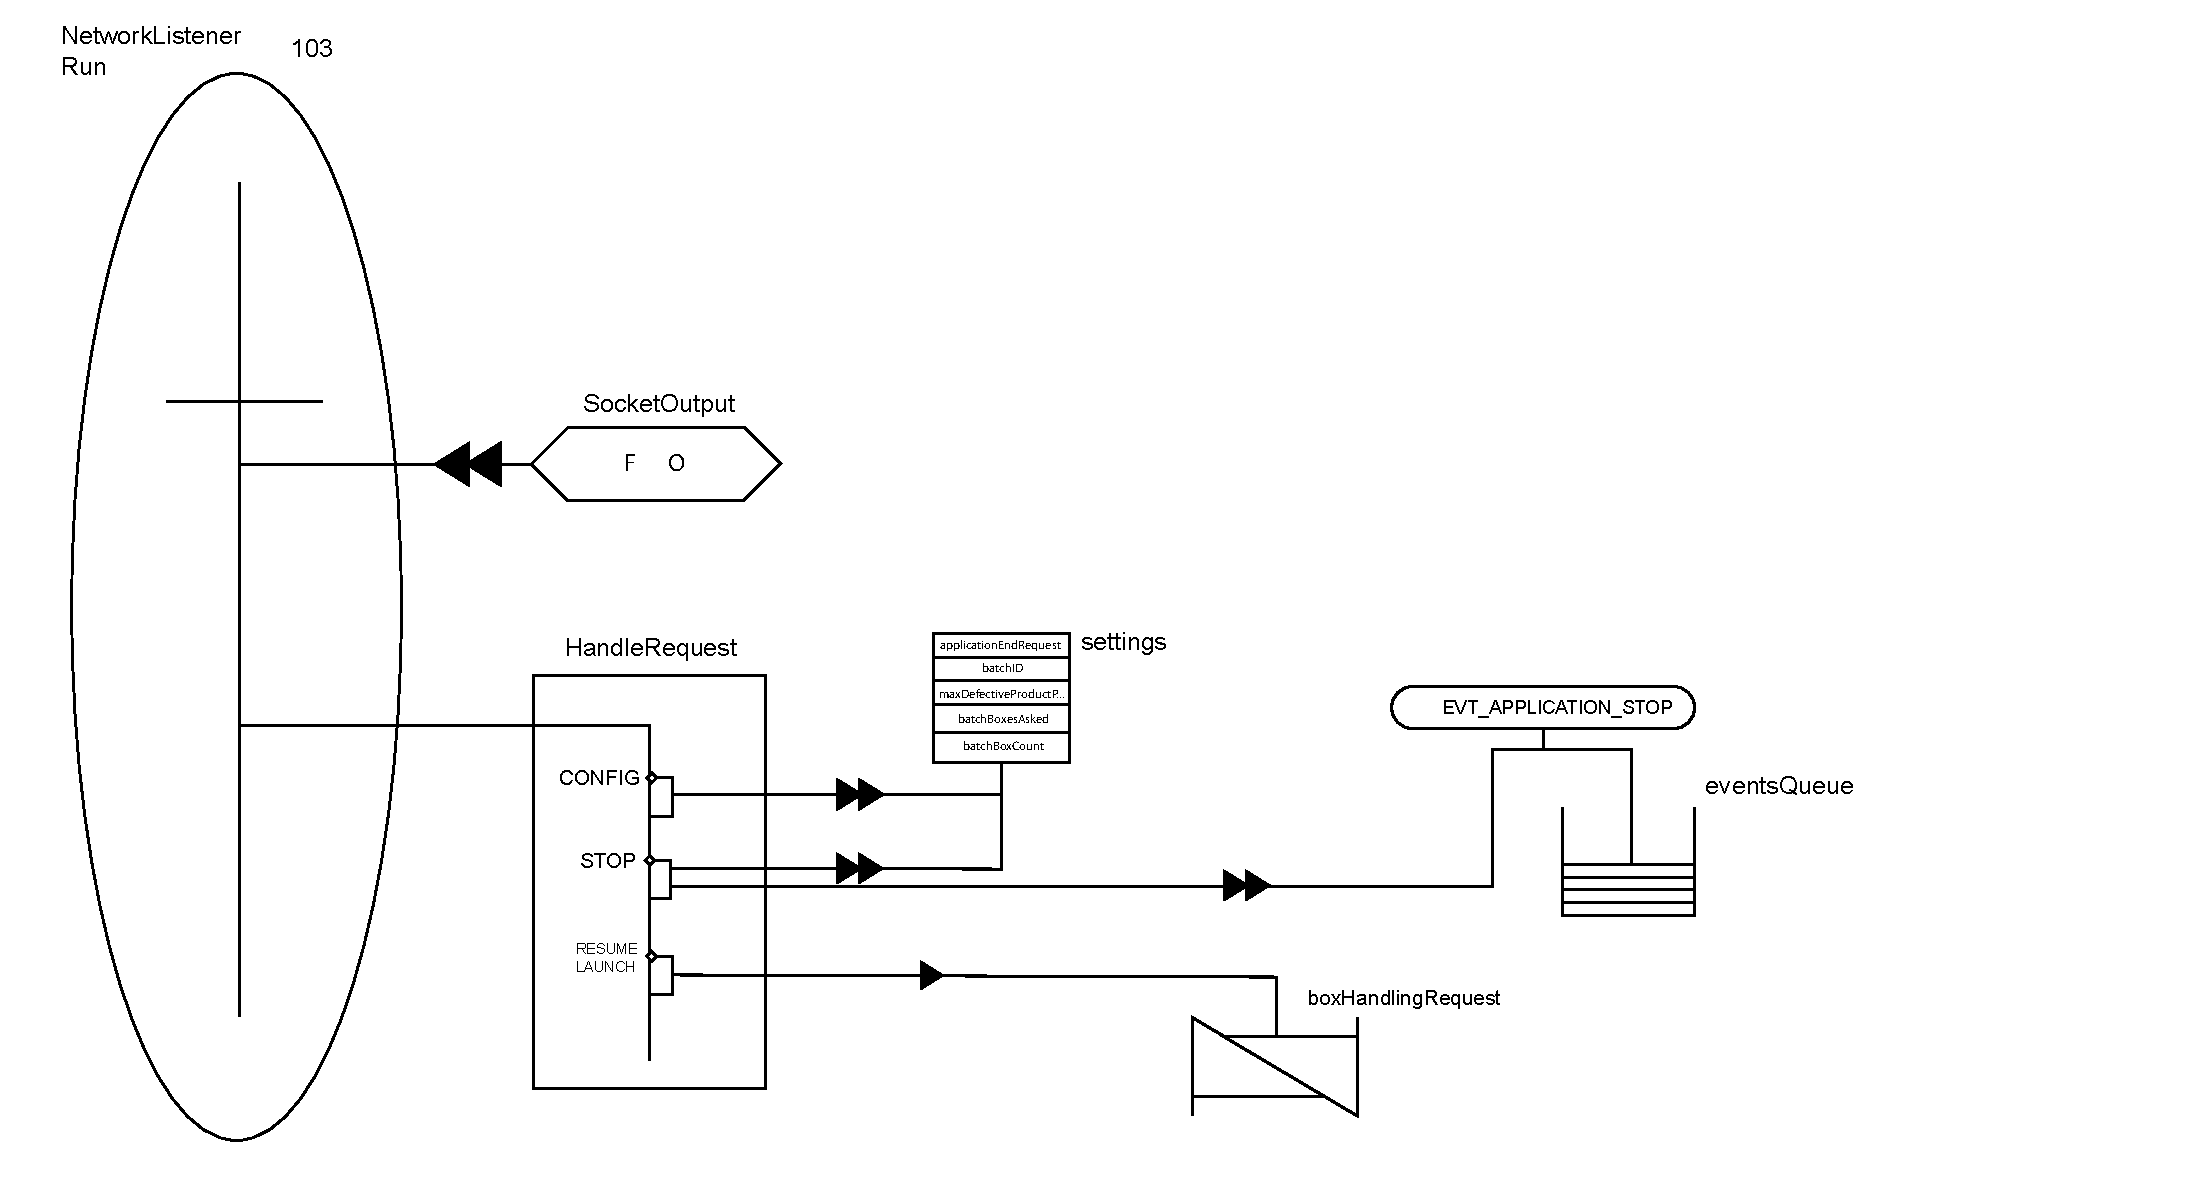
\includegraphics[width=\textwidth]{../../SchemasLCG/NetworkListener-run.pdf}
	\end{frame}

	\subsection{Protocole en sortie}
	\begin{frame}
		\begin{enumerate}
			\item \texttt{REJECTED} : nombre de pièces ayant un défaut.
			\item \texttt{ACCEPTED} : un carton a été accepté par le système. Un argument pour indiquer le nombre de pièces.
			\item \texttt{LOG} : l'argument est un message à afficher.
			\item \texttt{ERROR} : erreur critique nécessitant une intervention. Un argument pour le code d'erreur.
			\item \texttt{WARNING} : erreur non critique (panne d'imprimante).
		\end{enumerate}
	\end{frame}

	\begin{frame}
	    \frametitle{LCG : EventManager : réseau en sortie}
	    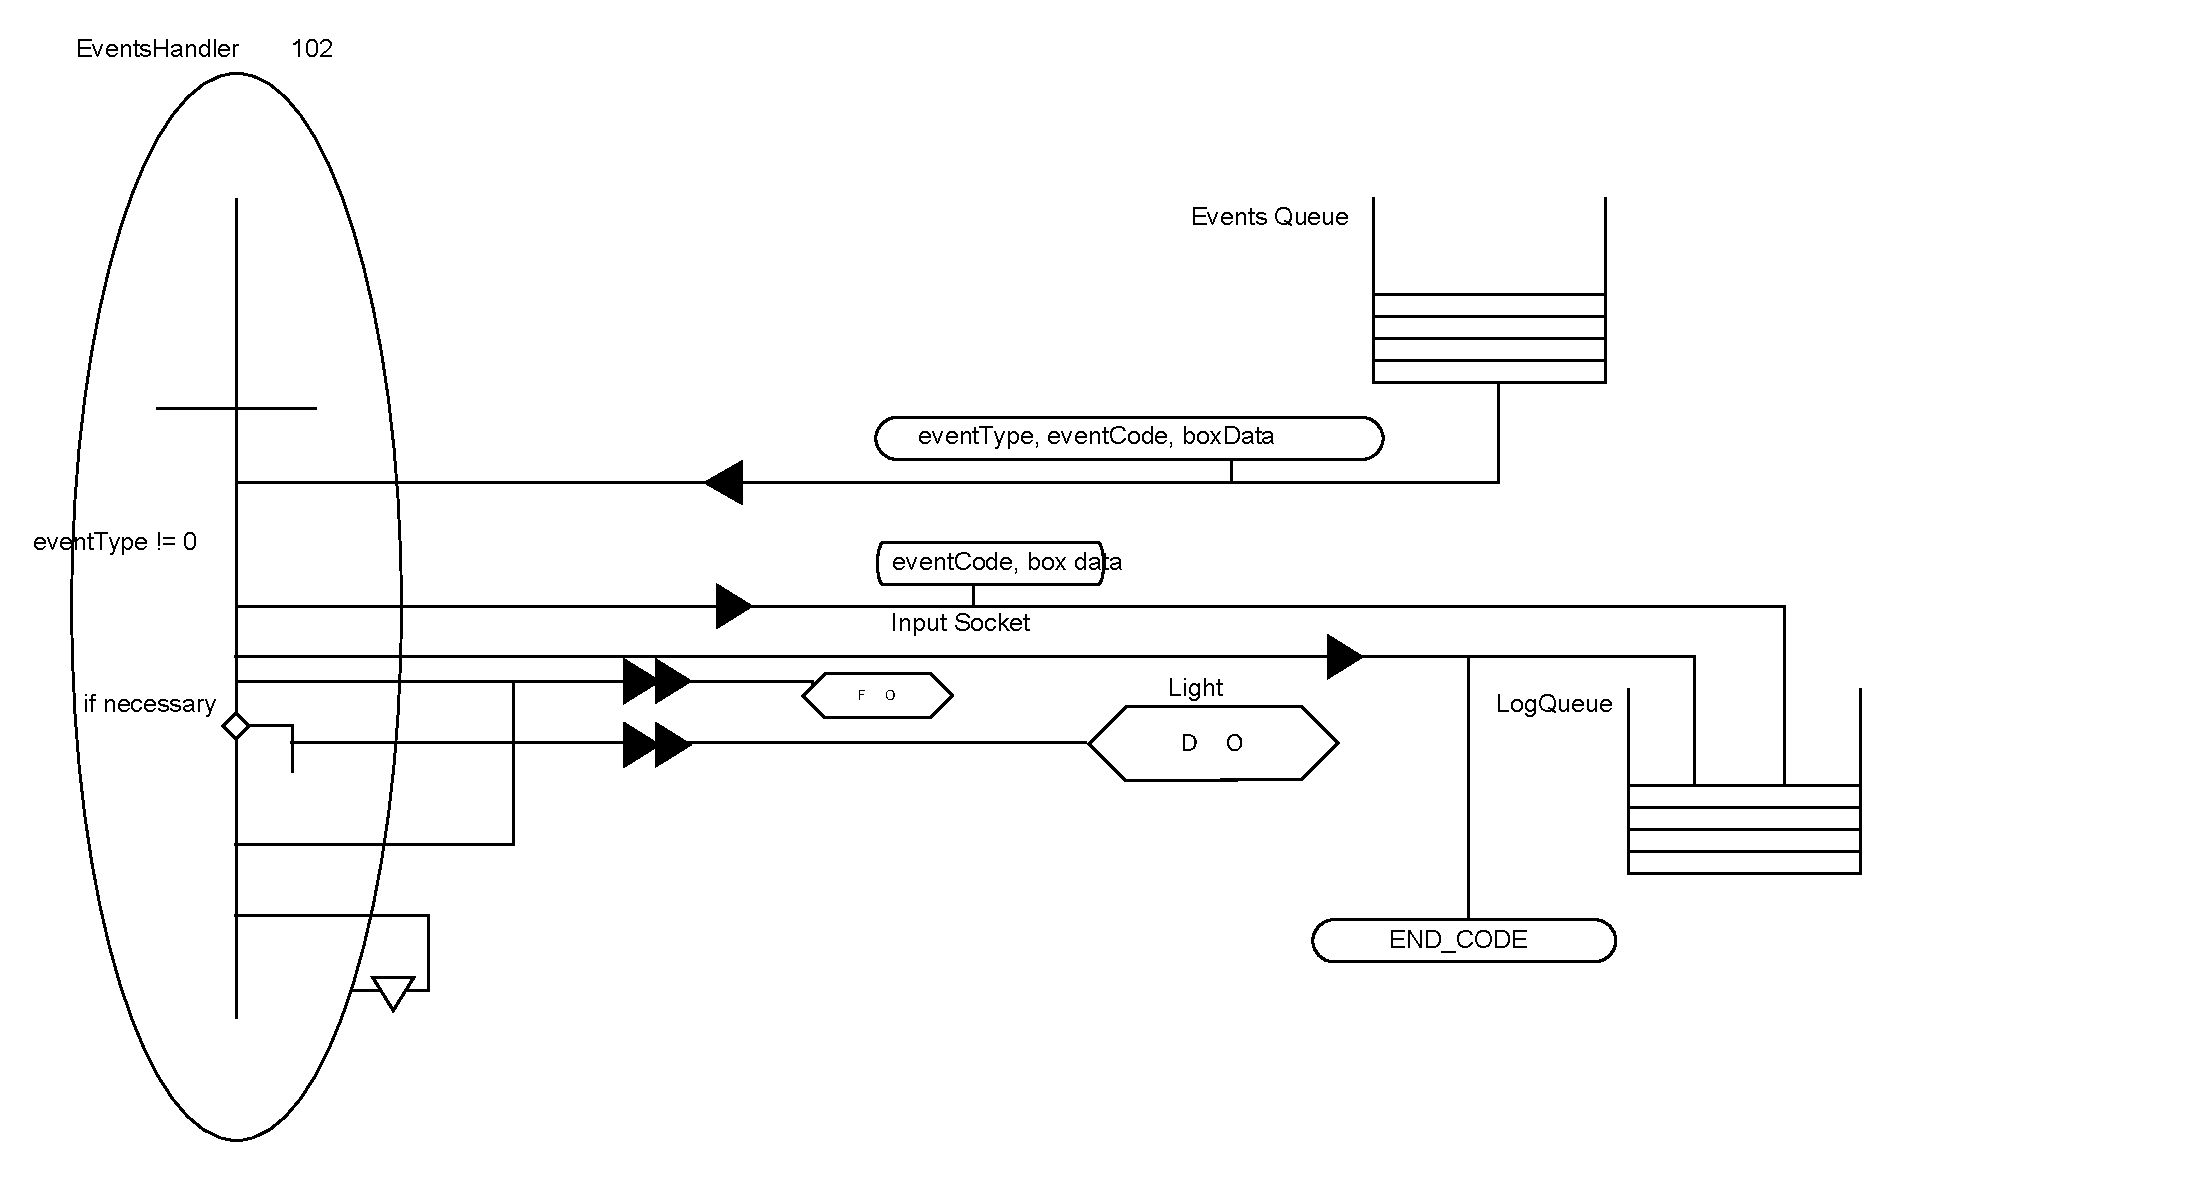
\includegraphics[width=\textwidth]{../../SchemasLCG/src/EventsManager.pdf}
	\end{frame}

	\begin{frame}
	    \frametitle{LCG : Journalisation sur disque}
	    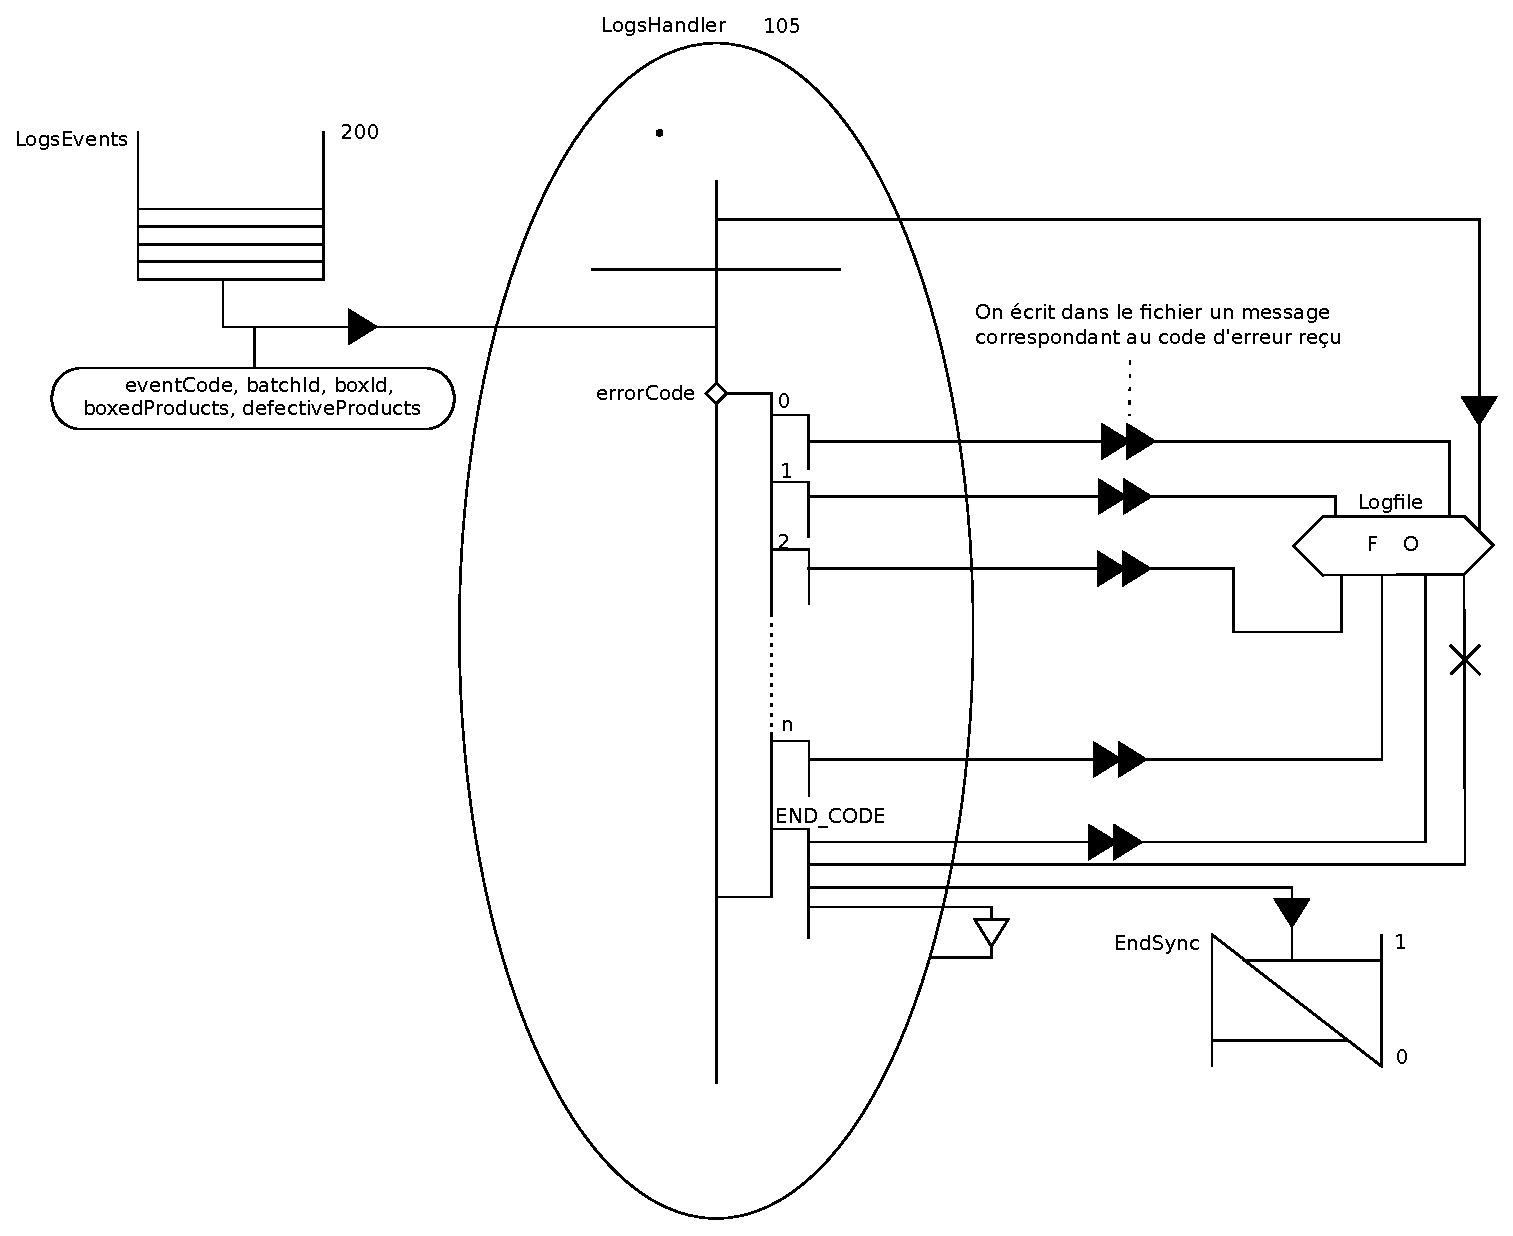
\includegraphics[width=0.8\textwidth]{../../SchemasLCG/LogsManager.pdf}
	\end{frame}


\section{Binôme 3 (Martin, Etienne)}
	\begin{frame}
	\begin{center}
		\frametitle{Lot 3 : Tâche mère}
		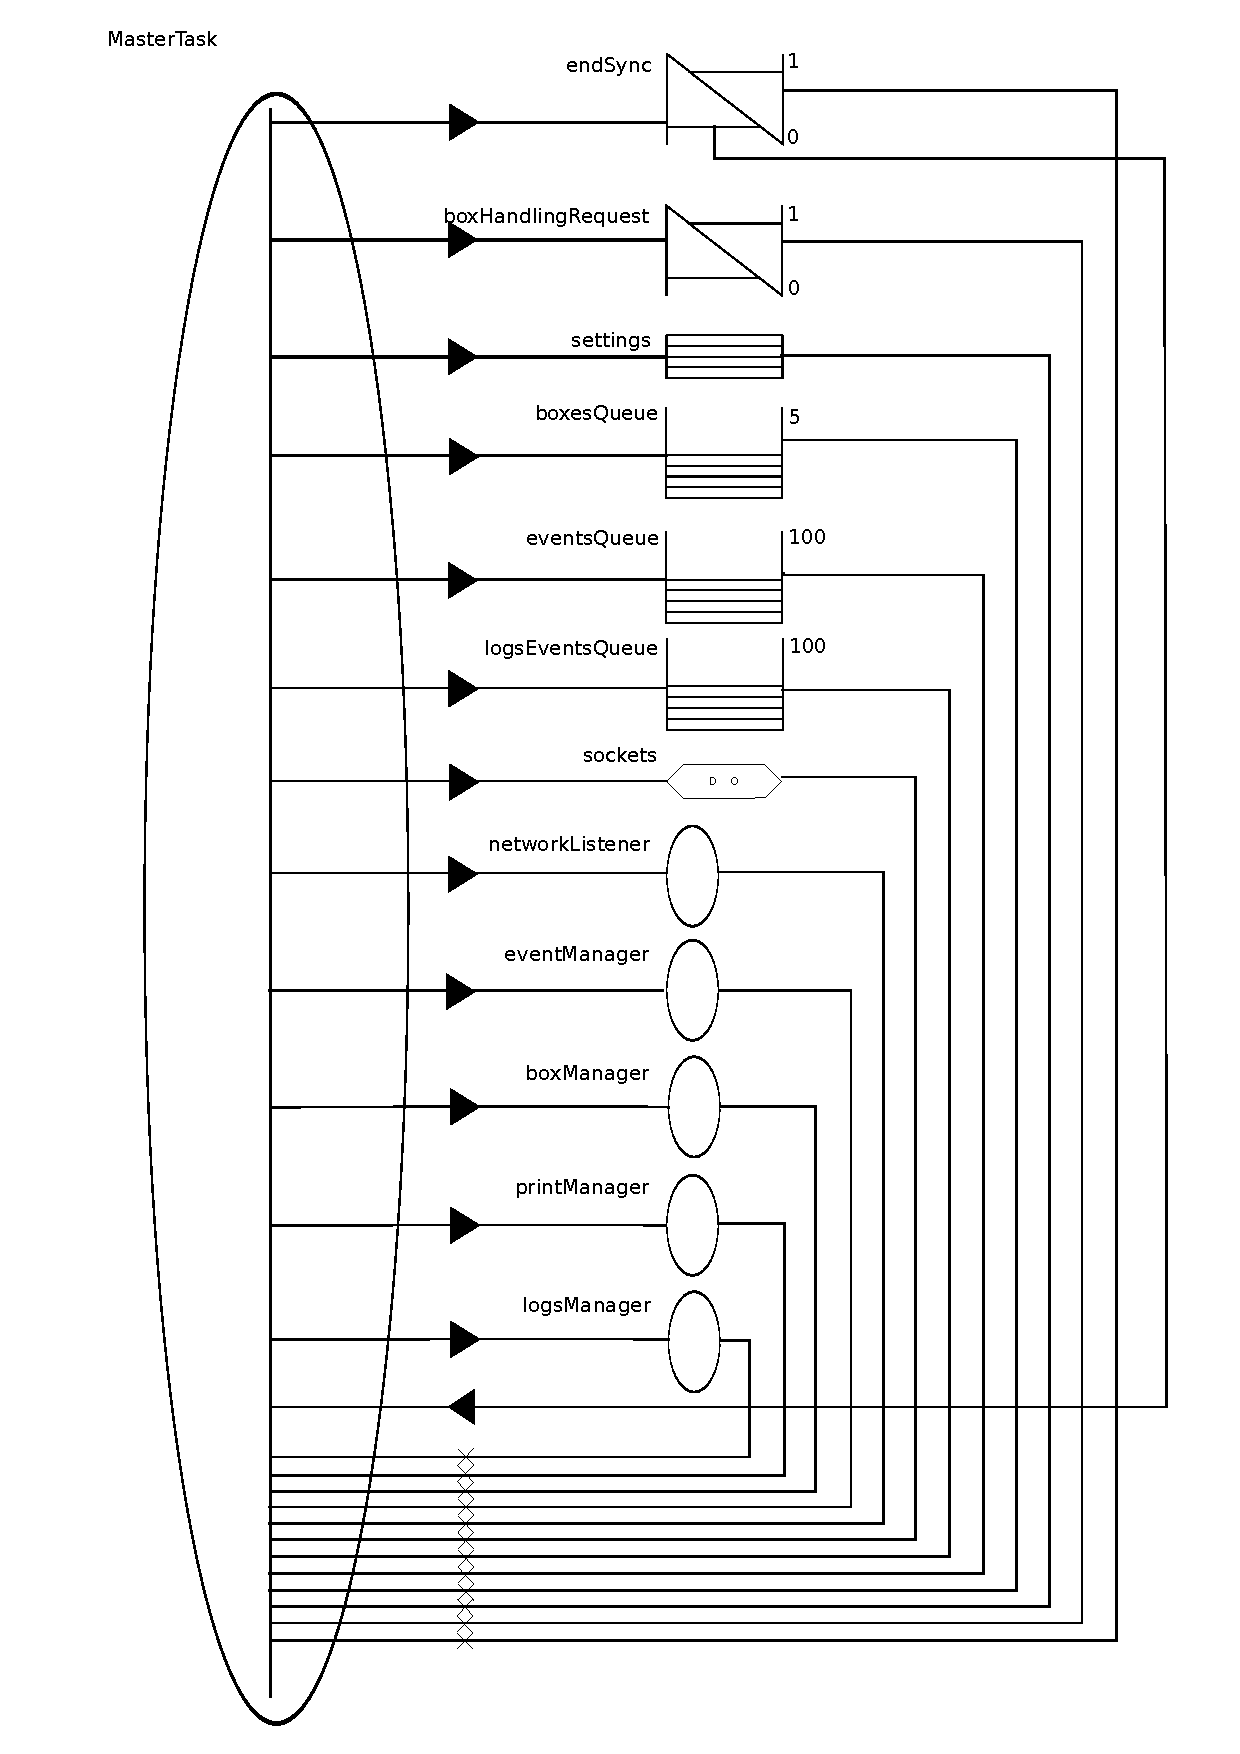
\includegraphics[height=0.8\textheight]{../../SchemasLCG/masterTask.pdf}
	\end{center}
	\end{frame}

	\begin{frame}
		LCG détaillé et complet en mode simulation
	\end{frame}

	\begin{frame}
		justification des choix effectués pour la simulation 
	\end{frame}

\section{Intégration}
	\begin{frame}
		Intégration
		\begin{itemize}
			\item démarche
			\item plan
			\item tests
			\item resultats
		\end{itemize}
		%TODO
	\end{frame}

	\begin{frame}
		démonstration de vos réalisations
		%TODO démonstration externe au slides ?
	\end{frame}

	\begin{frame}
		bilan du projet
		\begin{itemize}
			\item auto-critique
			\item améliorations possibles
			\item points forts/faibles
			\item difficultés rencontrées ...
		\end{itemize}
		%TODO
	\end{frame}

\end{document}

